\subsection{Application Architecture} \label{sec:application_architecture}
While the application is only designed as proof of concept, the structure of it is not random. Given that it acts as an example implementation, it is designed to demonstrate how the server functionality can be used for an application. The game is coded as an Android application. As many other types of software, there is different versions of Android, and when deciding which version to target, one should usually consider that anyone using older versions will be excluded from using the application. Given that the developed application is not meant for release, this concern has been disregarded. As such the application is developed for a somewhat newer version of Android called "Jelly bean" (Version 4.1 or alternatively API level 16). This version was announced on June 27th, 2012\cite{jelly-bean}. This potentially allows for easier programming as a newer version can mean both additional features and bugfixes.

The application is built using standard Android activities, described in \ref{subsec:components}. These activities represent one screen layout each - For example a login screen or a lobby screen for a game. The exact coupling and flow of these activities can be seen in figure \ref{fig:appstructure}. The idea is that after login, the user has a menu from where the application branches out, providing the option to create, join or resume a game.
What is not shown in the figure is that the user can still use the Android "back" button. Rather than just exiting the application when this is pressed, the application has been designed to go back in logical steps, depending on where the user is in the application. When creating, joining, resuming or playing a game, using the back button will lead back to the Menu screen, allowing the user to pick something else to do. Using the button from the Menu logs the user out, displaying the login screen, and from here it will exit the application.

\begin{figure}[H]
\centering
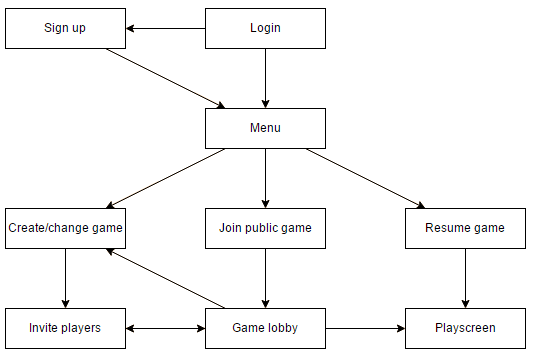
\includegraphics[width=\textwidth]{billeder/appstructure.png}
\caption{Structure of the application}
\label{fig:appstructure}
\end{figure}

\subsection{Coupling with Server Functionality} \label{subsec:server-coupling}
With the exception of the Menu, all activities require communication with the server. To facilitate this communication easily, several classes are used for this in the application, among those the \textit{Client} and a series of classes for handling XML. These are described in the paragraphs below. For a visualization of the structure in which they are used, see figure \ref{fig:appcommunication}.

\paragraph{Client}
The Client class is responsible for all communication with the server. The Client is thin and therefore, its implementation is very simple. The advantage of this is easier porting of the client to other platforms since the less code the client contains, the less coding is required to rewrite during a port.\\

It connects to the server upon being instantiated and is then able to send and receive strings using methods called \textit{send} and \textit{read}. For any desired server functionality, the programmer should use the send method. Given that the string sent is readable by the server, this will prompt the server to perform the requested action, and send a response to the client. To get this answer, the programmer should use the read method to retrieve the returned XML string.

\paragraph{XML Libraries}
The server accepts some pre-defined XML strings to understand commands sent from the client. The reasoning behind this is described in section \ref{subsec:interfaces}. For a programmer it can be tedious to write up XML strings manually in the different activities. To ease this process, some static classes were created to assist the generation of these strings. \textit{EncodeServerXML} and \textit{EncodeActionXML} handles the parsing of arguments into the XML format. \textit{EncodeServerXML} parses requests for management such as login, game creation and requesting a list of public games, while \textit{EncodeActionXML} handles actions for the games themselves such as updating coordinates and shooting people.

The classes take a number of arguments, for example a username and password to create a login request. This is then parsed into a XML format that the server can read and returned. The programmer must then utilize the Client class to send the created request. This exact usage can be seen in figure \ref{lst:facadepattern}.

Similar to the encoding classes, are matching classes for decoding, namely \textit{DecodeServerXML} \textit{DecodeActionXML}. These are able to take XML strings and decode variables into proper Java types. When the server receives a login request, it will attempt to find a matching user in the database. If it succeeds it will return the ID of the user, along with a "TRUE" message, indicating that the login was a success. It is however returned as an XML string, which is why the decoding classes can ease the process by extracting the ID and message.

To further ease the creation of XML strings, a trivial helper class, \textit{Tag} was created. It is simply able to create opening and closing tags, removing the need to manually enter parts of the XML strings. It is used by calling \textit{Tag.open()} or \textit{Tag.close}, passing the name of the tag that should be handled. Passing the string \textit{abc} to the two methods would produce the strings \textit{<abc>} and \textit{</abc>} respectively.

\begin{figure}[H]
\centering
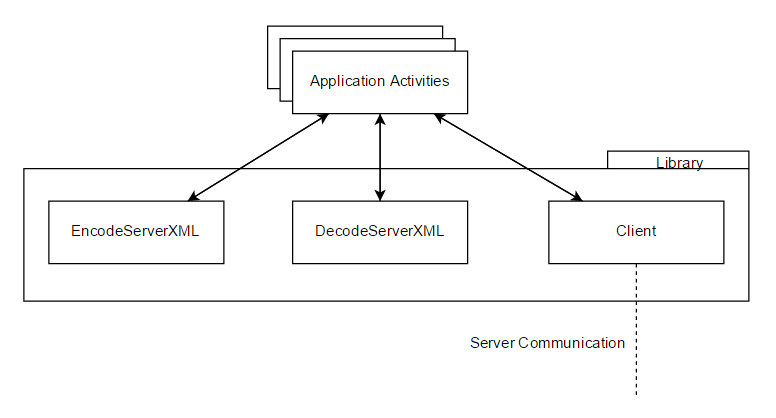
\includegraphics[width=\textwidth]{billeder/appcommunication.png}
\caption{Handling of server communication}
\label{fig:appcommunication}
\end{figure}